\chapter{Identifying Key Traits}
In this particular task, we aim to identify what are the most important signals strongly related to university degree holders. To identify these signals, we will treat this task as a predictive modelling problem. The first step is to prepare dataset which includes creating the train and test sets. Next, a simple learning classifier will be trained on the dataset the features are information about the individuals (demographics, tools used, company info etc.) and the target determines if the individual completed the university degree or not. All of the features and the target are binary. After the model is trained with a decent evaluation metric score, the important features of the model are obtained using Permutation Importance. These features provide some sense about their importance with an order or ranking.
\begin{listing}[!htpb]
    \inputminted{octave}{Code/traits.m}
    \caption{Identifying key traits of university degree holders.}
    \label{listing:traits}
\end{listing}

\begin{listing}[!htpb]
    \inputminted{octave}{Code/trait-print.m}
    \caption{Classifier Accurary}
    \label{listing:accuracy}
\end{listing}
The classifier shows a decent accuracy score of about 80\%, let's now look at the permutation importance of every variable.

\begin{figure}[!ht]
    \centering
    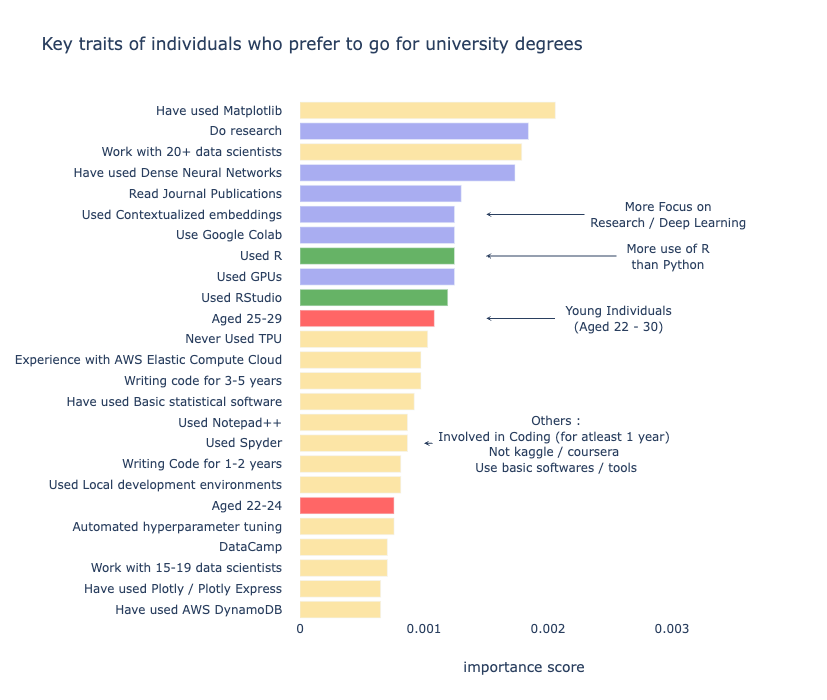
\includegraphics[width=\linewidth]{Figures/Outputs/traits.png}
    \caption[Traits of individuals]{Key traits of individuals who prefer to go for university degrees.}
    \label{fig:figure-13}
\end{figure}
The chart shows a few interesting traits of people associated with university degrees: More use of R than Python, More focus on research and deep learning, mainly young individuals (aged 22-30), involved in coding for at least a year, not doing kaggle or MOOCs.

\chapter{Conclusion}
The main focus of this analysis was to understand and evaluate if there are any significant differences in the self-taught scientists and university degree holders. The insights presented in this notebook, convey a broad message about the importance of "masters in data science degrees". We can observe that it is not impossible to achieve certain job roles or position and even compensation without any degree in data science/analytics. In Section 4 we saw that there are as many as self-made data scientists (without any degree) earning similar compensation as with the degree holders. The case is not just restricted to the USA but also true in many other countries. This means that organizations value skills and talent over any degree, that's why they pay huge chunks of money for that skill. We also observed that there are no major distinctions in the type of work individuals in this field do on a daily basis, everyone has to spend a good amount of time in data analysis and cleaning, There are almost equal percentage of respondents who build machine learning services, prototypes and also do experimentation.

It might be wrong to strongly say that it’s not worth it all. There are many positives associated with it as well: One can get edge during job hunt over those who do not have masters degree, one can establish their network with professors, fellow students, and industry partners, one can get exposure to many new areas, and can polish a lot of skills. Academic institutions are responding to a market demand and generating programs, due to it. It is possible that what students learn might be very different from what a data scientist does.
\newpage
Jeremy Howard said the following in a \href{https://www.reddit.com/r/Futurology/comments/2p6k20/im_jeremy_howard_enlitic_ceo_kaggle_past/cmty7kf/}{reddit AMA}:
\begin{importantbox}
    There is nothing that you could learn in a master of computer science that you could not learn in an online course, or by reading books. However, if you need the structure or motivation of a formal course, all the social interaction with other students, you may find that useful. I think that online courses are the best way to go if you can, because you can access the world's best teachers, and have a much more interactive learning environment — for example the use of short quizzes scattered throughout each lecture. Specifically, the courses that I would recommend our the machine learning course on Coursera, the introduction to data science course on Coursera, and the neural networks for machine learning course — surprise surprise, also on Coursera! Also, all of the introductory books here are a good choice. The most important thing, of course, is to practice download some open datasets from the web, and try to build models and develop insights, and post them on your blog. And be sure to compete in machine learning competitions — that's the only way to know whether your approaches are working or not.
\end{importantbox}
The key takeaway is that one can become a data scientist (or any other similar position in this field) with right skills and can also manage to get decent compensation even without going through "Masters in Data Science (or similar degrees)". There are many alternatives - Coursera, Kaggle, Udemy, Udacity, eDX, Linkedin Learning, Fast.ai to name a few. These resources are either completely free or are much cheaper than dedicated university degrees. Additionally, one can complete these courses in a much shorter time as compared to the university courses. If there are any other reasons for the desire to pursuing masters, example - personal goals, passion, interest, utilizing the breaks etc, one should consider pursuing university courses.

If someone is thinking of getting a degree, in data science, analytics, just because they have the time and money to spare, is not wise. If the interest in analytics is driven by the desire for a job that offers better rewards than what they are getting now, then one should look for alternative paths to make that career move. \href{https://www.forbes.com/sites/metabrown/2016/07/29/4-reasons-not-to-get-that-masters-in-data-science/#4813020640c0}{Meta S Brown} from Forbes says, "At the end, we need to remember that Data Scientist is a Title. Many give themselves or have this title because that's the work they do, not because they have a particular degree".

It's just about taking the first step, start studying from online courses, do relevant projects, start making kaggle contributions, and keep improving your resume and profile. In the end, whatever path someone takes, they will most likely produce similar outcomes. The following Sankey depicts this message very well.
\begin{figure}[!ht]
    \centering
    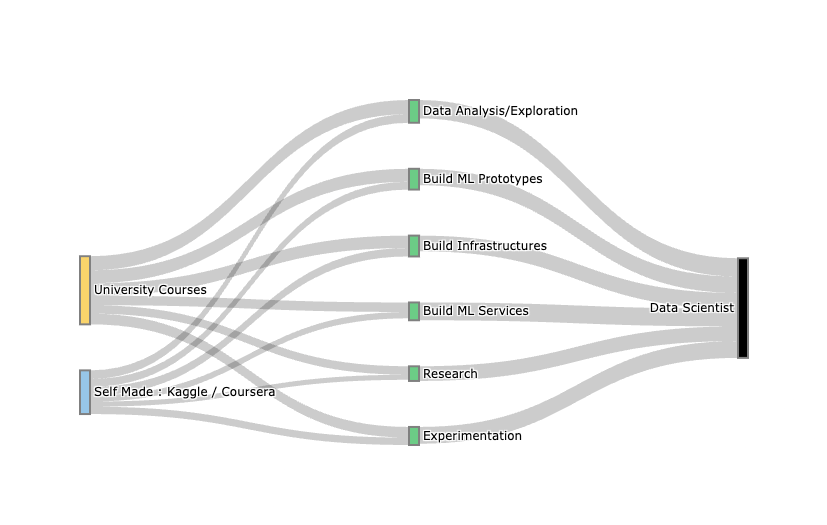
\includegraphics[width=\linewidth]{Figures/Outputs/sankey.png}
    \caption[Sankey diagram showing demographic of data scientists]{Sankey diagram showing the distribution of data scientists with and without university degrees.}
    \label{fig:figure-14}
\end{figure}

\section*{Summary}
\begin{itemize}
    \item If someone wants to learn data science skills only, then no its not worth it because there are many excellent free / cheaper alternatives on the internet. Kaggle is an excellent place to start.
    \item If someone wants to work as a data scientist (fresher or career change), then it may or may not be worth it because there is no gurantee that one will get a data science job after the university degree. A non degree holder with right skillset, right experience, and right attitude may get a better job than the one with a degree title.
    \item If someone wants to earn more, then it is not necessary to have university degree, as one with good experience or good skills can grab very high compensation packages.
    \item If someone wants to do more research, then it may be worth it given that one chooses a right specialization.
    \item If someone is passionate to learn more and gain exposure then it is definately worth it. University degree can provide a platform to network, participate in different events, and improve the foundation.
\end{itemize}